% Chapter 

\chapter{Findings, Conclusion, Limitations and Recommendation} % Main chapter title

\label{Chapter10_conclusion-recommendation} % For referencing the chapter elsewhere, use \ref{Chapter10} 

\section{Introduction }
 The goal of this chapter is to  provide the findings, conclusion, limitations  and recommendations for future research. 
 In \nameref{Research findings} (section \ref{Research findings}), 
 I provide the findings of the research relevant to the research question. 
 In \nameref{Research Conclusions} (section \ref{Research Conclusions}), 
 I have listed the conclusions from the viewpoint of rigor and relevance.
 In \nameref{Research Limitations} (section \ref{Research Limitations}), 
 I have listed the limitations of my research.  
 In \nameref{Future Recommendations} (section \ref{Future Recommendations}),
 the possibilities of exploration in this technology has been highlighted.
 
 
 \section{Research findings}\label{Research findings}
 There was one research question in chapter  \ref{Chapter4_problem-domain}, \nameref{Chapter4_problem-domain} section \ref{Research Question} and four sub-research questions in section \ref{Sub-research question}. Answers to these research questions listed in below section.
 
 \subsection{Research Question 1}
 \textbf{What  are  elements  for  a  cyber news feed  assessment  method  and  what  are  the parameters for automation?}
 \subsubsection{Answer}
The most important element for a cyber newsfeed assessment is the collection of cyber newsfeed items, followed by other methods as mentioned below and configuration of stakeholders specific tags in the tool is key to the automation. 

 \subsubsection{Sub-Research Question 1a}
\textbf{What are the core core concepts of cyber newsfeed and how do they work according to literature?}

\bigbreak

\textbf{Answer: } The core concepts around the cyber newsfeed are about the sources of the newsfeed, 
then the processes like collection, processing, analysis of the newsfeeds. 
In chapter \ref{Chapter7_literature-review},  \nameref{Chapter7_literature-review}
(section \ref{Existing practices, systems, and people involved in automated cyber newsfeed}), 
the essentials concepts according to the literature review has been provided in detail.
Chapter \nameref{Chapter7_literature-review}  also illuminate the related concepts of people and practices
(subsection \ref{Existing-practices}) in link with these processes. 

 
\subsubsection{Sub-Research Question 1b}
\textbf{How does the vendor field of automated cybernewsfeed suppliers of artefacts look like according to the literature?}

\bigbreak

\textbf{Answer: } This study looked at 17 different threat intelligence tools in chapter \ref{Chapter7_literature-review}, \nameref{Chapter7_literature-review} (TABLE \ref{tab:tip-list}) provided by the different vendors. Among the tools, the collection of data is the only common behaviour. Other downstream activities like processing and analysis require customisation and configuration organisation-specific newsfeeds. The answer to this question is  in chapter \ref{Chapter7_literature-review}, \nameref{Chapter7_literature-review} (subsection \ref{Existing systems}).
 



 \subsection{Research Question 2}
 \textbf{How to make a prototype to filter contextual cyber Intelligence,
 perform automatic relevance tagging and 
 perform analysis for risk determination and advisory?}
 
\begin{figure}[ht]
\centering
    \fbox{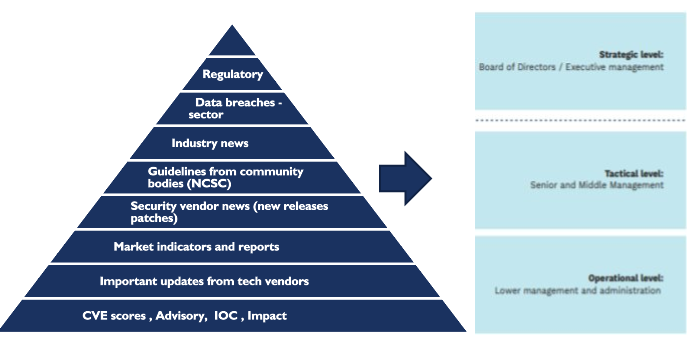
\includegraphics[width=.85\linewidth]{Figures/tailored.PNG}}
    \caption{Organisation-specific cyber newsfeeds to stakeholders}
    \label{fig:tailored}
\end{figure}
 \subsubsection{Answer}
There are three modules designed to achieve this, 1) the Collector, 2) the Processor and 3) the Analyser\&Advisory. 
A cyber analyst can pre-configure the required parameters of sources, contexts and tags with the help of a GUI. 
For writing advisory and editorial checks, the work flow has been proposed and a diagram has been provided for reference. 
The details are mentioned in chapter \ref{Chapter8_artefact-design},
\nameref{Chapter8_artefact-design}
(section \ref{Artefact and Artefact breakdown}). 
These three modules are: 
 

\begin{enumerate}
    \item \textbf{Collection Module:} 
    After evaluating 17 tools, 
    FreshRSS tool was used for collecting the newsfeed from various sources. 
    FreshRSS is an open source collection tool for RSS feeds and 
    can ingest cyber newsfeeds from multiple sources. 
    It has a GUI, has a database, is easy to deploy and is easy to customise.  

    \begin{figure}[ht]
    \centering
        \fbox{
\includegraphics[width=.75\linewidth]{Figures/freshrss.png}}
        \caption{FreshRSS for Cyber newsfeed collection }
        \label{fig:freshrss}
    \end{figure}

    \item  \textbf{Processor Module: }
    For configuring the context specific to an area of particular interests of a stakeholder. 
    In this research we have filtered the first level of information 
    based on the contextualisation of Vendor and Non-Vendor specific information's.
    After filtration, 
    the relevant tagging was done by the tool with the vendor name, 
    for example TAG = Cisco, Microsoft or Amazon. 
    Tagged values of a particular interests of a stakeholder has been shown as a JavaScript Object Notation (JSON)  output with an example. 
    A JSON\footnote{JSON is a file format defined at \url{https://en.wikipedia.org/wiki/JSON}} 
    output of this processor module can be found
    in table format in Appendix \ref{json}. 
    The source code for archiving old data(cyber newsfeeds) collected  by the collector module is attached in Appendix \ref{AppendixChapter8} (section \ref{tag-archiving}).
    In Appendix \ref{AppendixChapter8} (section \ref{filter-context}), the SQL source code for filtering contextual data can be found. 
    For tagging of the more specific tags to a specific cyber newsfeed item, the PL-SQL function can be found in Appendix \ref{AppendixChapter8} (section \ref{tag-addtag}).
    To publish the processed cyber newsfeed via RSS feed to a cyber analysts, the source code can be found at \ref{AppendixChapter8} (section \ref{rss-send}).
    
    \item  \textbf{Analysis \& Advisory Module:}
    This module is designed to work with the output from the processor module and is human intensive. 
    First it will make correlations between similar cyber newsfeed items 
    either manually or automatic with the help of machine learning algorithms. 
    Then the cyber analysts, 
    using their skills and knowledge will perform additional research and provide additional information about the related risk and an advisory to act. 
     Finally the gathered cyber newsfeed contents will be validated together with editorial experts before dispatching the cyber intel to the stakeholders.

 \end{enumerate}


 \subsection{Research Question 3}
 
 \textbf{How to make a prototype for assessing the quality of the data sources?}
 \subsubsection{Answer}
 As mentioned in chapter 
 \ref{Chapter7_literature-review}, \nameref{Chapter7_literature-review}, 
 there are six qualitative 
 (TABLE \ref{table:qualitative}) 
 and ten quantitative 
 (TABLE \ref{table:quantitative}) 
 ways to evaluate the quality of cyber newsfeed sources. 
 The quantitative metrics will gain prominence over qualitative methods.
This has been explained in chapter \ref{Chapter7_literature-review} (section \ref{Existing methods available for data source quality assessment}).
 
In this research we have finalised one quantitative method \enquote{\textit{Extensiveness: Evaluates   how   many optional parameters are filled in}} as mentioned in   
TABLE \ref{table:source-quality} 
of 
chapter
\ref{Chapter8_artefact-design}, 
\nameref{Chapter8_artefact-design}.
In addition to 
\enquote{\textbf{Extensiveness}} 
as quantitative method, 
the Focus group suggested to capture the stakeholder's direct feedback as an evaluation parameter for cyber newsfeed source quality.

 \subsection{Research Question 4}
 \textbf{How to get the prototype validated for \emph{both 1) the design and 2) the output of this artefact} by the end users of specific organizations?}
 \subsubsection{Answer}
The prototype was validated by the Focus group using GSS, The chapter \ref{Chapter9_artefact-evaluation}, \nameref{Chapter9_artefact-evaluation},
lists the results of the  validation. 

\section{Research Conclusions} \label{Research Conclusions}
In this section, I presented my research conclusions.
My main conclusions are based 
upon the analysis of 
the collected research data. 
I categorized my conclusions as follows: 
1) first part on the relevance for the stakeholders and 
2) second part on the rigor applicable to this artefact 
\enquote{Cybernewsfeed technology}. 

\subsection{Conclusions on the relevance of the \enquote{Cybernewsfeed technology}}

%As mentioned in chapter \nameref{Chapter6_research-approach} my research needs to be relevant.
Below are the conclusions on the relevance of the 
\enquote{Cybernewsfeed technology} provided by the stakeholders 
in the Group Support System (GSS) sessions.

Outcome of the GSS was that the stakeholders indicated 
that getting organisation-specific information via the cyber newsfeeds
is important to them (section \ref{sec:interest}). 
The proposed tool  
\enquote{Cybernewsfeed technology} was regarded as fullfilling
this need (\ref{sec:concept}).

Outcome of the GSS was that the stakeholders currently do not use
similar technology to fulfill their need (section \ref{ref:familiar}).
The stakeholders stated that they would purchase similar technology
if it was available to them (section \ref{sec:pay}).

For the technology itself to be relevant to the stakeholders, 
it needs to provide information on a daily basis
with exception of the critical information.
Notification of critical information needs to be real-time 
to be relevant to the stakeholders (section \ref{sec:frequency}).
Real-time notification is preferred 
by the stakeholders via instant messaging (section \ref{sec:media}). 

%The topic of data privacy and data security has the main interest with the stakeholders (section \ref{sec:desire}).


 %\subsubsection{Relevance Conclusion 1} 
 %The results indicate that getting organisational-specific cyber newsfeeds is eminent   for the stakeholders and there is a need of similar technology like this tool \enquote{Cybernewsfeed technology}.  
    

%\subsubsection{Relevance Conclusion 1} According to the target group exercise that we did, actionable cyber intel is important for the stakeholders because of the .....

%\subsubsection{Relevance Conclusion 2} 
%Based on the feedback on interests from the stakeholders. 
%From an organizational point of view, 
%they are knowing but they don't use it yet, 
%so there is a need.

%\subsubsection{Relevance Conclusion 3}
%The stakeholders are willing to pay  money 
%but they are not yet using a similar service.

%\subsubsection{Relevance Conclusion 4} 
%The stakeholders that I have interviewed during the GSS are looking forward to more strategic and tactical news, rather than the operation news. This could be a case because they functional at strategic and tactical level and they have more need for strategic and tactical level of information.

%\subsubsection{Relevance Conclusion 5} 
%Most desirable frequencies to receive such a cyber neewsfeed is daily. 
%The stakeholders want to receive the information in real time for the %critical cyber newsfeed.

%\subsubsection{Relevance Conclusion 6}
%According to the target group exercise, the most desired media is messaging. 

%\subsubsection{Relevance Conclusion 7} 
%Data privacy is perceived as the most 
%important concerns for the stakeholders.

\subsection{Conclusions on the rigor of the \enquote{Cybernewsfeed technology}}




%\subsubsection{Rigor Conclusion}



In my literature research I found a limited amount of
academic sources on the topic of cyber intelligence 
within the scope of my research.
My research is a contribution to the existing body of knowledge.
The insight that the solutions similar to \enquote{Cybernewsfeed technology: REVEAL}
requires organisation-specific configuration and that the solution
needs editorial functionalities to tailor the content,
are an addition 
to the existing body of knowledge.

%There are very few academic research done in cyber intel because I did not find many literatures. 
%I made a contribution in adding a new knowledge source by concluding that such cyber intel sharing technologies like \enquote{Cybernewsfeed technology: REVEAL} requires  organisation-specific configurations functionalities and in built editorial functionalites to tailor the content of newsfeeds. 
%Optimum output from the \enquote{Cybernewsfeed technology} can be achieved with the help of configurable parameters and custom defined algorithms.



According to my literature research and stakeholders feedback only tools capabilities are not sufficient to deliver organisation-specific newsfeeds, a role of the cyber analyst and editor are also very critical.
%for the analysis and providing any applicable solution for the specific cyber news feed intel.

%It can be concluded that there are some important factors to consider when designing and developing the 
%\enquote{Cybernewsfeed technology} 
%for optimum output. 

%\subsubsection{Rigor Conclusion 4}
%There are two configurable tasks required to run this tool. 1) Configuration of data sources and 2) configuration of tags required to filter the specific items. 



\section{Research Limitations}\label{Research Limitations}

%\subsection{Limitation 1}
Prototype on assessing the data source quality in chapter \ref{Chapter8_artefact-design} section \ref{quality_source} could not be implemented or validated. There was not enough data and time to assess the quality information of the cyber newsfeed sources. 

%\subsection{Limitation 2}
%The technology needs more functional and technical capabilities to be %operational and a productive product. 


%\subsection{Limitation 3}
%To calculate automated risk determination, 
%implementation of decision tree 
%is required and has not been covered in this paper.

%\subsection{Limitation 4}
%The Graphical User Interface (GUI)\footnote{GUI according to Wikipedia \url{https://en.wikipedia.org/wiki/Graphical_user_interface}} in this artefact may not be acceptable by the users, as it is only for demonstration and can be improved with better screens.

%\subsection{Limitation 2}
The Focus group has six participants for the representation of stakeholders population.
One could argue if six participants are enough,
where I think the level of expertise of the participants
is more important then the amount of participants.

%\subsection{Limitation 3}
The research has been executed in coordination with one organisation  instead of multiple organisations, I could have collected more requirements for the artefact.


%\subsection{Limitation 4}
The research was executed in six months and I feel I could have done better with more time and due to less time the results of this tool has not been used in a real life environment, 
the tool is still in incubation phase. 

%\subsection{Limitation 5}
I am a software developer and not a cybersecurity expert,
but when I started my research, slowly learned and gained the knowledge in the field of cybersecurity, 
 and this improved my research work.



\section{Recommendations for future research}
\label{Future Recommendations}


The curiosity to understand the missing influence of such tools among the stakeholders could be an interesting illumination.
To me this is an indication that there is a need that is not yet met. 
It is my recommendation to further study the root cause of this need
with the stakeholders.
I  would also recommend to improve the prototype 
and develop it in an iterative software development way into a more mature solution.

Another direction could be to improve the maturity of the solutions 
by combining both cyber security and software Engineering knowledge, for example to implement `automatic risk analysis and determination` or `automatic source sanitation`.
%In my opinion, by adding this knowledge can  
%done in the scientific way that I used in my research.
 

\section{Personal Reflection}


I have learned a couple of things about myself during my
Executive Master education at the Antwerp Management School. 
Knowledge wise I have gained a broader and holistic view on the IT related corporate practices; 
and have learned to apply academic and holistic approach to any problem. 
I learned to be resilient during the thesis, 
improved myself in adverse situations, 
for instance I lost my new job, had hopes in future so started to learn new technologies, and then the continuous learning has became a part of me.

I never considered myself as a good writer, 
never wrote more than two pages in English. 
I had problem understanding Dutch, but things have changed; I can write a fair amount of literature, can converse in Dutch language. 
I am also reflecting on my presentation to the CEO and learnt that I should prepare such meetings better and not getting distracted before the critical presentations.

\newpage
\centering \section*{Thankyou}
\centering \subsection*{With the feeling of being thankful}
 \begin{figure}[htbp!]
    \centering
        \fbox{
\includegraphics[width=.20\linewidth]{Figures/namaste.png}}
        \caption{}
        \label{fig:namaste}
    \end{figure}
\FloatBarrier




